\section{目的與講義要求}

依講義 PDF 第 107--110 頁，網表 01 重現圖 26.1 同型動態電路直接串接的錯誤；02 依圖 26.4/26.5 加入相同 10 fF 耦合雜訊並掃描強度；03 回答問題 1 的速度比較。三份網表共 9 個分析，均完成且無 error 或 failed measurement。模擬器仍回報加密區塊的警告內容被隱藏，不能將其解讀為模型完全無警告。

\section{電路、測試條件與判讀}

以提供模型、1.0 V、25°C 為教學條件，並非已認證額定電壓或原講義 2.5 V 製程重現。除網表另註，Wn/Wp/L = 0.6/1.8/0.25 µm，輸出負載 5 fF；時脈週期 10 ns、邊緣 20 ps。採 0.2/0.8 V 作明列的低／高判讀準則；這是本報告診斷門檻，並非已萃取接收器雜訊容限。

同型 N-domino 使用兩個四電晶體動態 NAND（第二輸入固定高），每級接靜態反相器；N-P 鏈則直接串接四個 N/P 動態級。各鏈完成相同的非反相邏輯，輸出負載相同；N-domino 共 12 顆、N-P 鏈共 16 顆核心電晶體。這是照講義拓樸比較，並非相同電晶體數或最佳化邏輯努力的比較。

所有網表只保留 \texttt{MODEL\_SETUP\_REQUIRED} 註解；執行前須自行補入本機模型設定。公開檔案不含模型內容或載入路徑。圖由實際列印資料重繪，逐案例 CSV 與量測 JSON 置於 \texttt{results/}。

\section{步驟 1：錯誤串接}

輸入 A 在預充相位先升高。時脈於 2.5 ns 上升時，X 與 Y 初始均高，第二級先被 X 打開；即使第一級隨後把 X 放低，Y 已流失的電荷在評估相位沒有主動充回路徑。7 ns 的 Y = 0.655339 V，未達 0.8 V 的高電位診斷門檻。本模型下是顯著高電位劣化，並非完整放到 0 V；如實保留此差異。

\begin{figure}[htbp]\centering
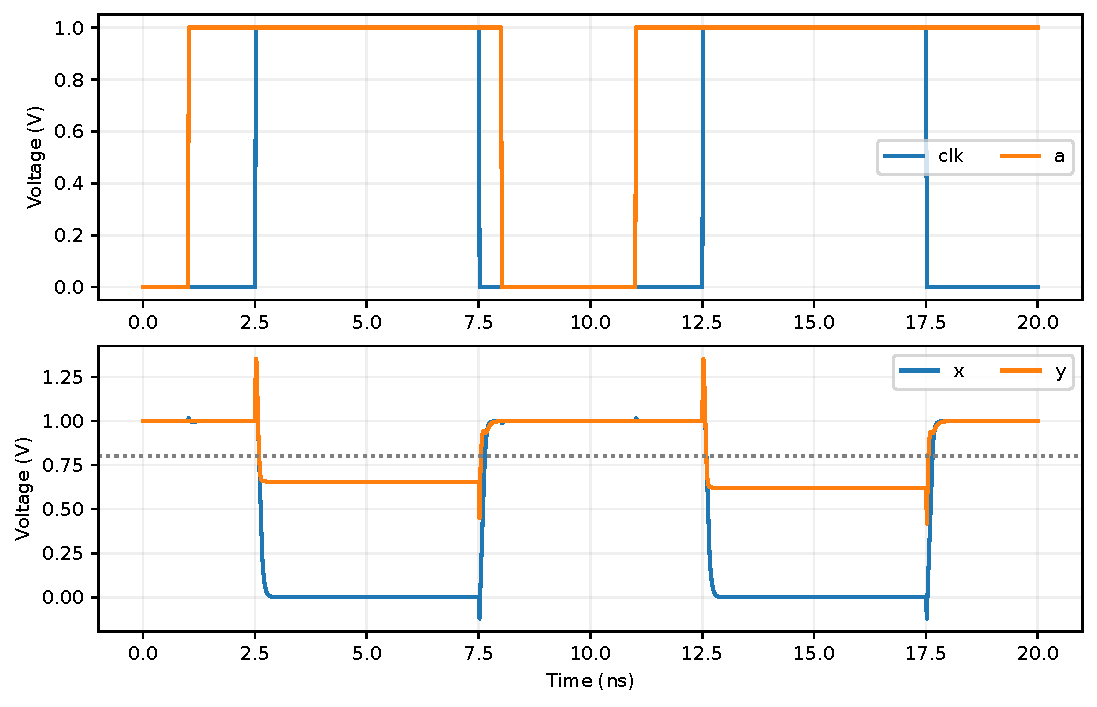
\includegraphics[width=.93\linewidth]{figures/unsafe_cascade.pdf}
\caption{直接串接的電荷流失；虛線為 0.8 V 診斷線。}
\end{figure}

\section{步驟 2：相同雜訊比較}

A 固定 0，預期兩鏈輸出皆低。在評估相位中，aggressor Q 於 4 ns 從 1 降到 0 V，經相同電容耦合至各鏈第一動態節點；10 fF 為講義條件。N-domino 的靜態反相器抑制小擾動，而 N-P 級的輸入直接控制對向 MOS，較小的浮接節點變化就可能被後級再生。

\begin{center}\small
\begin{tabular}{lrr}
\toprule
C (fF) & N 峰值 (V) & N-P 峰值 (V) \\
\midrule
0.001 & -0.000011 & -0.096783 \\
2 & 0.000056 & -0.096796 \\
5 & 0.000141 & -0.096797 \\
10 & 0.000249 & 0.999901 \\
15 & 0.000443 & 1.000282 \\
20 & 1.006744 & 1.001090 \\
30 & 1.010412 & 1.001674 \\
\bottomrule
\end{tabular}
\end{center}

\begin{figure}[htbp]\centering
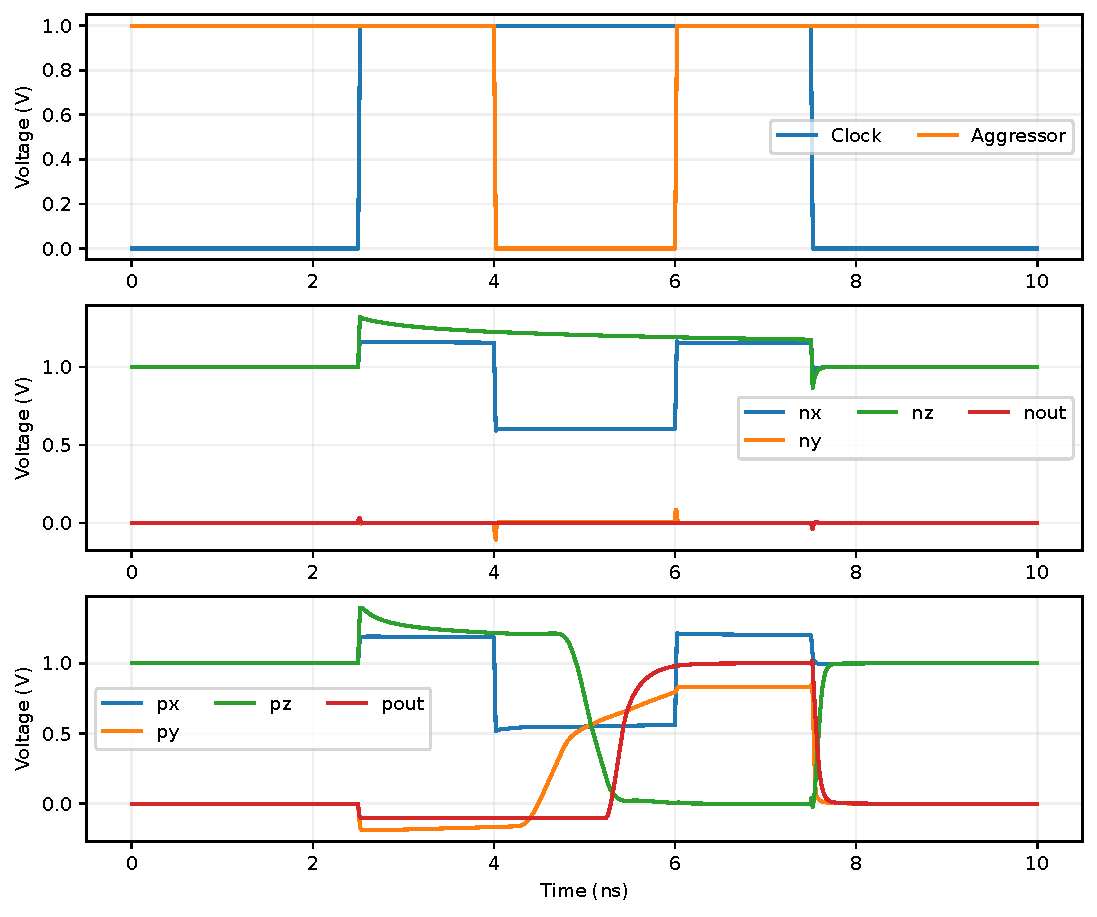
\includegraphics[width=.93\linewidth]{figures/equal_noise.pdf}
\caption{10 fF 下的相同擾動與各鏈內部節點。}
\end{figure}

10 fF 時，N-domino 峰值只有 0.000249 V，N-P 輸出卻約為 1 V，出現持續的錯誤高電位。15 fF 仍有同樣區別；20/30 fF 時兩者都失敗。接近零耦合的 0.001 fF 對照組顯示 N-P 輸出約 -0.097 V 的 clock feedthrough，沒有將其裁成理想 0 V。測試支持這組條件下 N-domino 抗擾動較佳，並不保證任意尺寸、斜率、負載或雜訊形式都如此。

\section{問題 1：速度與討論}

另以輸入在 4 ns、評估相位內由低轉高比較速度，避免把不同時脈預充時間算成資料延遲。以輸入與輸出 0.5 V 交越量測，N-domino 為 367.720 ps，N-P 為 657.328 ps。本實作 N-domino 較快；不能單憑 N-P 省掉靜態反相器就斷言其較快，因為 PMOS 動態堆疊驅動力、各節點負載與尺寸都參與延遲。

\begin{figure}[htbp]\centering
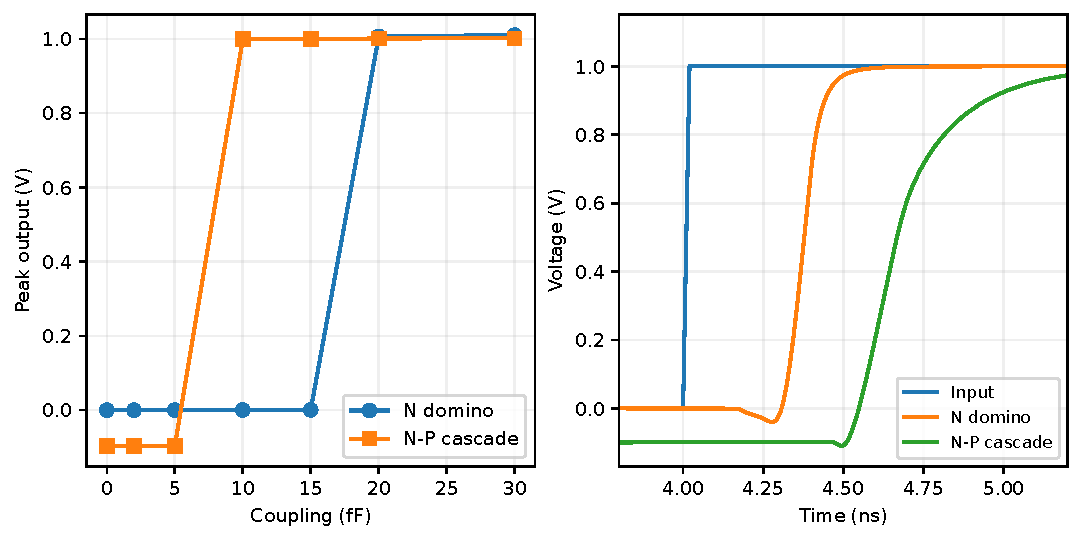
\includegraphics[width=.93\linewidth]{figures/sweep_and_speed.pdf}
\caption{左：耦合掃描；右：無耦合電容的資料速度測試。}
\end{figure}

預充輸出不可打開後級的評估路徑，這是安全串接的核心條件；同型需插反相器，異型可直接相接，但後者的類比雜訊容忍仍需實測。所有結果皆為有限條件的電路模擬，未宣稱 PVT、版圖後或完整雜訊簽核。
